\section{Pianificazione}
\textit{TechSweave} ha deciso di pianificare il progetto in base alle scadenze sotto riportate. Di conseguenza il progetto è stato suddiviso nelle seguenti fasi:
\begin{itemize}
    \item Analisi;
    \item Consolidamento dei Requisiti;
    \item Progettazione architetturale;
    \item Progettazioni di dettaglio e codifica;
    \item Validazione e collaudo;
\end{itemize}
Ognuna di queste fasi verrà suddivisa in attività da realizzare entro i tempi stabiliti per la fase stessa e sarà mostrata nei rispettivi diagrammi di Gantt\textsubscript{\textbf{G}}.
\subsection{Analisi}
\textit{Periodo: dal 2021-03-11 al 2021-04-02}
Questo periodo corrisponde alla data di formazione del gruppo e termina con la data ultima per la consegna dei documenti relativi alla \textit{Revisione dei Requisiti}.\\
Questa fase è stata scomposta nelle seguenti attività che corrispondono ai documenti prodotti:
\begin{itemize}
    \item \textbf{Studio di Fattibilità:} viene effettuato uno studio dei capitolati comprendente i lati positivi e negativi a essi collegati, per poi selezionarne uno. L'attività è bloccante per l'\textit{Analisi dei Requisiti v2.0.0};
    \item \textbf{Norme di Progetto:} vengono specificate tutte le regole da rispettare durante lo sviluppo del progetto. Da questo documento dipenderanno le norme di stesura di tutti i prodotti successivi;
    \item \textbf{Analisi dei Requisiti:} vengono studiati e analizzati i requisiti legati al capitolato scelto nello \textit{Studio di Fattibilità v1.0.0};
    \item \textbf{Piano di Progetto:} il presente documento in cui attività, compiti e risorse precedentemente analizzate vengono distribuite tra i membri del team. Nel seguente documento è presente il calcolo del preventivo per la realizzazione del progetto;
    \item \textbf{Piano di Qualifica:} vengono individuati i metodi necessari per garantire la qualità del prodotto;
    \item \textbf{Glossario:} documento contenente tutti i termini che possono risultare ambigui durante lo svolgimento del progetto, di essi viene fornita una definizione sintetica ma esaustiva.
\end{itemize}
\begin{figure}[!ht]
    \caption{Diagramma di Gantt della fase di Analisi}
    \vspace{5px}
    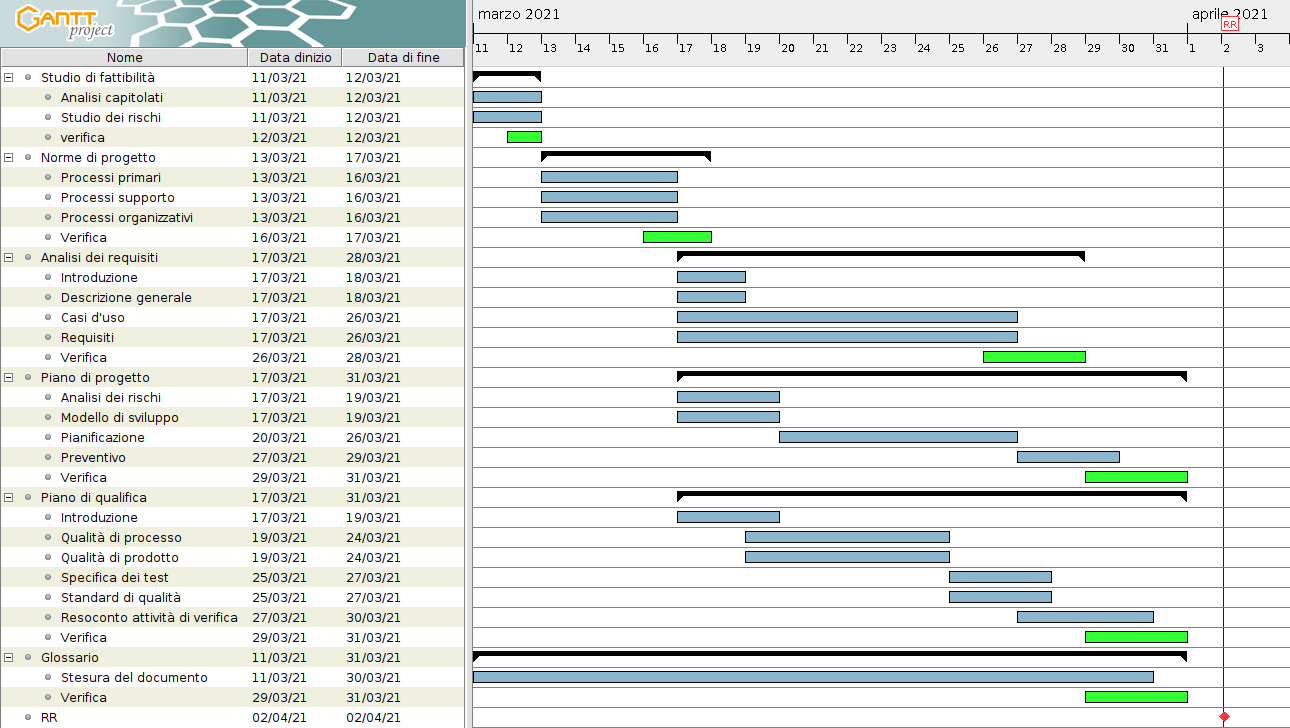
\includegraphics[scale=0.21]{../../../Images/Diagrammi/Gantt/diagramma_gantt_analisi_0.2.png}
    \centering
\end{figure}

\subsection{Consolidamento dei requisiti}
\textit{Periodo: dal 2021-04-02 al 2021-04-09}\\
Questa fase comincia con la fine di quella di Analisi e termina il giorno della presentazione della \textit{Revisione dei Requisiti}. Le attività di questa fase sono:
\begin{itemize}
    \item \textbf{Consolidamento:} con lo scopo di consolidare e migliorare i requisiti ottenuti nella fase precedente;
    \item \textbf{Preparazione alla presentazione:} per preparare il materiale necessario alla presentazione del 2021-04-09;
    \item \textbf{Incremento e Verifica:} nella quale vengono migliorati i documenti prodotti nella fase precedente se necessario;
    \item \textbf{Approfondimento personale:} ogni componente del gruppo dovrà dedicare delle ore di studio autonomo e approfondimento riguardo alle tecnologie necessarie per sviluppare il prodotto.
\end{itemize}
\begin{figure}[!ht]
    \caption{Diagramma di Gantt della fase di consolidamento dei requisiti}
    \vspace{5px}
    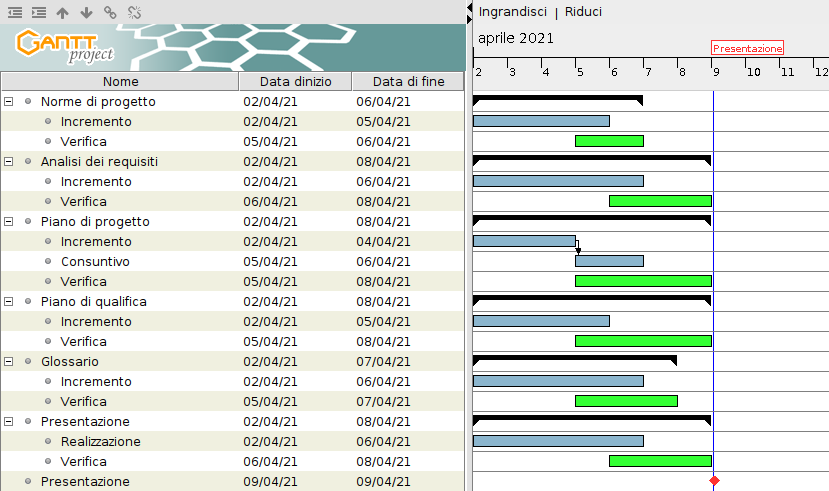
\includegraphics[scale=0.4]{../../../Images/Diagrammi/Gantt/consolidamento.png}
    \centering
\end{figure}

\subsection{Progettazione architetturale}
\textit{Periodo: dal 2021-04-09 al 2021-05-03}\\
Questa fase comincia il giorno successivo alla presentazione e la sua fine coincide con la data di consegna della \textit{Revisione di Progettazione}. In questo lasso di tempo verrà individuata una soluzione architetturale che soddisfi i requisiti richiesti.\\
Le attività di questa fase sono:
\begin{itemize}
    \item \textbf{Incremento e verifica:} in cui i documenti precedentemente redatti vengono aggiornati e migliorati;
    \item \textbf{Technology Baseline\textsubscript{\textbf{G}}:} viene fatta un'analisi ad alto livello per comprendere appieno le tecnologie coinvolte, scegliendo l'architettura del codice e i design pattern\textsubscript{\textbf{G}} che saranno adoperati per lo sviluppo. Viene codificato il Proof of Concept\textsubscript{\textbf{G}} che sarà presentato o condiviso tramite repository con committente e proponente per verificare il corretto sviluppo del software.
\end{itemize}
\begin{figure}[!ht]
    \caption{Diagramma di Gantt dell'attività di progettazione architetturale}
    \vspace{5px}
    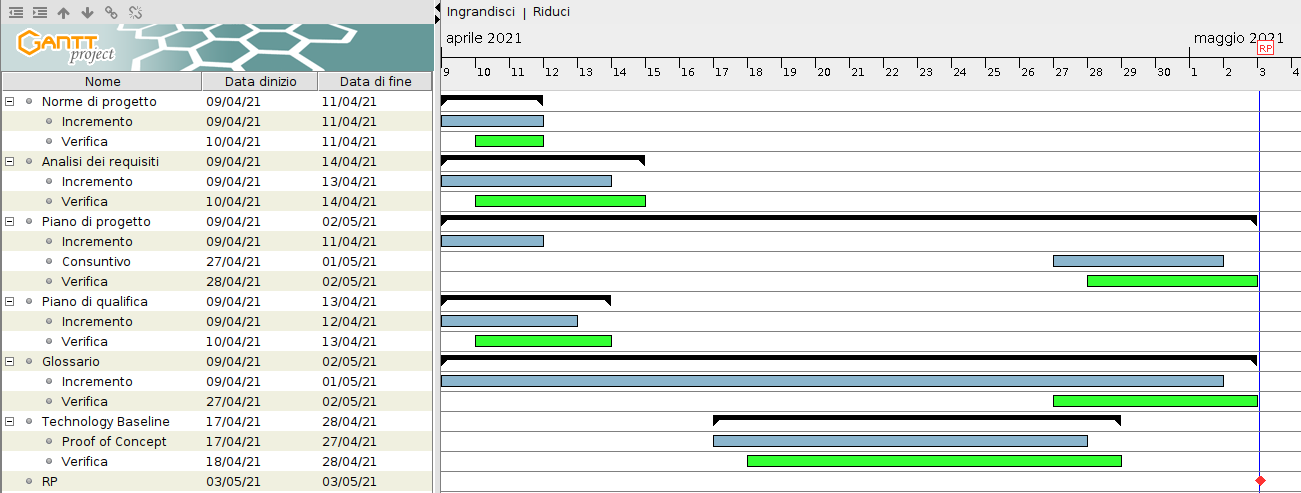
\includegraphics[scale=0.3]{../../../Images/Diagrammi/Gantt/progettArchitetturale_v2.png}
    \centering
\end{figure}

\subsection{Progettazione di dettaglio e codifica}
\textit{Periodo: dal 2021-05-10 al 2021-06-04}\\
L'inizio di questa fase è il giorno della scadenza della \textit{Revisione di Progettazione} e la data di fine coincide con la data di consegna dei documenti in vista della \textit{Revisione di Qualifica}.\\
Le attività di questa fase sono suddivisi in sei incrementi di sviluppo, per ognuno dei quali sono riportate le seguenti voci:
\begin{itemize}
    \item obbiettivi
          \begin{itemize}
              \item software;
              \item documentali;
          \end{itemize}
    \item periodo;
    \item ruoli attivi;
    \item attività previste;
    \item diagrammi di Gantt
\end{itemize}


\subsubsection{Incremento 6}
\subsubsubsection{Obbiettivi}
Gli obbiettivi che il gruppo di pone di soddisfare in questo periodo sono i seguenti:
\begin{itemize}
    \item Preparazione alle attività di progettazione e codifica di dettaglio;
    \item Incremento della documentazione per verifica e miglioramento continuo.
\end{itemize}
\subsubsubsection{Periodo}
Il gruppo ritiene che per il raggiungimento degli obbiettivi serviranno tre giorni di lavoro;\\
Il periodo interessato sarà dal 2021/05/10 al 2021/05/12
\subsubsubsection{Ruoli Attivi}
Per la realizzazione di questi obbiettivi il gruppo ritiene che saranno attivi i seguenti ruoli:
\begin{itemize}
    \item \textit{Responsabile di progetto};
    \item \textit{Amministratore di progetto};
    \item \textit{Analista};
    \item \textit{Progettista};
    \item \textit{Programmatore};
    \item \textit{Verificatore}.
\end{itemize}

\subsubsubsection{Attività previste}
Per soddisfare gli obbiettivi preposti il gruppo ritiene di dover svolgere le seguenti attività:
\subsubsubsection{Diagrammi di Gantt}

\subsubsection{Incremento 7}
\subsubsubsection{Obbiettivi}
Gli obbiettivi che il gruppo di pone di soddisfare in questo periodo sono i seguenti:
\begin{itemize}
    \item Miglioramento della struttura delle funzioni Lambda, con l'aggiunta dei filtri di ricerca;
    \item  Miglioramento delle chiamate \textit{API GATEWAY} nel frontend per ottenere le informazioni delle funzioni lambda;
    \item Inizio della stesura della documentazione legata al prodotto software;
    \item Incremento della documentazione per verifica e miglioramento continuo.
\end{itemize}
\subsubsubsection{Periodo}
Il gruppo ritiene che per il raggiungimento degli obbiettivi serviranno cinque giorni di lavoro;\\
Il periodo interessato sarà dal 2021/05/13 al 2021/05/17
\subsubsubsection{Ruoli Attivi}
Per la realizzazione di questi obbiettivi il gruppo ritiene che saranno attivi i seguenti ruoli:
\begin{itemize}
    \item \textit{Responsabile di progetto};
    \item \textit{Amministratore di progetto};
    \item \textit{Analista};
    \item \textit{Progettista};
    \item \textit{Programmatore};
    \item \textit{Verificatore}.
\end{itemize}

\subsubsubsection{Attività previste}
Per soddisfare gli obbiettivi preposti il gruppo ritiene di dover svolgere le seguenti attività:
\subsubsubsection{Diagrammi di Gantt}

\subsubsection{Incremento 8}
\subsubsubsection{Obbiettivi}
Gli obbiettivi che il gruppo di pone di soddisfare in questo periodo sono i seguenti:
\begin{itemize}
    \item Ristrutturazione dei servizi lato backend;
    \item Riconfigurazione del linter \textit{eslint};
    \item Correzione della documentazione in base alla RP;
    \item Incremento della documentazione per verifica e miglioramento continuo.
\end{itemize}
\subsubsubsection{Periodo}
Il gruppo ritiene che per il raggiungimento degli obbiettivi serviranno tre giorni di lavoro;\\
Il periodo interessato sarà dal 2021/05/18 al 2021/05/20
\subsubsubsection{Ruoli Attivi}
Per la realizzazione di questi obbiettivi il gruppo ritiene che saranno attivi i seguenti ruoli:
\begin{itemize}
    \item \textit{Responsabile di progetto};
    \item \textit{Amministratore di progetto};
    \item \textit{Analista};
    \item \textit{Progettista};
    \item \textit{Programmatore};
    \item \textit{Verificatore}.
\end{itemize}

\subsubsubsection{Attività previste}
Per soddisfare gli obbiettivi preposti il gruppo ritiene di dover svolgere le seguenti attività:
\subsubsubsection{Diagrammi di Gantt}

\subsubsection{Incremento 9}
\subsubsubsection{Obbiettivi}
Gli obbiettivi che il gruppo di pone di soddisfare in questo periodo sono i seguenti:
\begin{itemize}
    \item Implementazione gestione dell'accesso;
    \item Distinzione tra cliente e venditore;
    \item Implementazione lato frontend;
    \item Incremento della documentazione per verifica e miglioramento continuo.
\end{itemize}
\subsubsubsection{Periodo}
Il gruppo ritiene che per il raggiungimento degli obbiettivi serviranno due giorni di lavoro;\\
Il periodo interessato sarà dal 2021/05/20 al 2021/05/21
\subsubsubsection{Ruoli Attivi}
Per la realizzazione di questi obbiettivi il gruppo ritiene che saranno attivi i seguenti ruoli:
\begin{itemize}
    \item \textit{Responsabile di progetto};
    \item \textit{Amministratore di progetto};
    \item \textit{Analista};
    \item \textit{Progettista};
    \item \textit{Programmatore};
    \item \textit{Verificatore}.
\end{itemize}

\subsubsubsection{Attività previste}
Per soddisfare gli obbiettivi preposti il gruppo ritiene di dover svolgere le seguenti attività:
\subsubsubsection{Diagrammi di Gantt}

\subsubsection{Incremento 10}
\subsubsubsection{Obbiettivi}
Gli obbiettivi che il gruppo di pone di soddisfare in questo periodo sono i seguenti:
\begin{itemize}
    \item Completamento Checkout;
    \item Completamento carrello;
    \item Completamento pagina PDP;
    \item Incremento della documentazione per verifica e miglioramento continuo.
\end{itemize}
\subsubsubsection{Periodo}
Il gruppo ritiene che per il raggiungimento degli obbiettivi serviranno tre giorni di lavoro;\\
Il periodo interessato sarà dal 2021/05/22 al 2021/05/24
\subsubsubsection{Ruoli Attivi}
Per la realizzazione di questi obbiettivi il gruppo ritiene che saranno attivi i seguenti ruoli:
\begin{itemize}
    \item \textit{Responsabile di progetto};
    \item \textit{Amministratore di progetto};
    \item \textit{Analista};
    \item \textit{Progettista};
    \item \textit{Programmatore};
    \item \textit{Verificatore}.
\end{itemize}

\subsubsubsection{Attività previste}
Per soddisfare gli obbiettivi preposti il gruppo ritiene di dover svolgere le seguenti attività:
\subsubsubsection{Diagrammi di Gantt}

\subsubsection{Incremento 11}
\subsubsubsection{Obbiettivi}
Gli obbiettivi che il gruppo di pone di soddisfare in questo periodo sono i seguenti:
\begin{itemize}
    \item Completamento Homepage;
    \item Completamento PLP;
    \item Implementazione ricerca di un prodotto;
    \item Incremento della documentazione per verifica e miglioramento continuo.
\end{itemize}
\subsubsubsection{Periodo}
Il gruppo ritiene che per il raggiungimento degli obbiettivi serviranno 2 giorni di lavoro;\\
Il periodo interessato sarà dal 2021/05/24 al 2021/05/25
\subsubsubsection{Ruoli Attivi}
Per la realizzazione di questi obbiettivi il gruppo ritiene che saranno attivi i seguenti ruoli:
\begin{itemize}
    \item \textit{Responsabile di progetto};
    \item \textit{Amministratore di progetto};
    \item \textit{Analista};
    \item \textit{Progettista};
    \item \textit{Programmatore};
    \item \textit{Verificatore}.
\end{itemize}

\subsubsubsection{Attività previste}
Per soddisfare gli obbiettivi preposti il gruppo ritiene di dover svolgere le seguenti attività:
\subsubsubsection{Diagrammi di Gantt}

\subsubsection{Incremento 12}
\subsubsubsection{Obbiettivi}
\begin{itemize}
    \item Completamento pagina venditore;
    \item Aggiunta sezione per la gestione delle categorie;
    \item Aggiunta visualizzazione elenco clienti e ordini ricevuti;
    \item Aggiunta sezione per la gestione di un prodotto;
    \item Incremento della documentazione per verifica e miglioramento continuo.
\end{itemize}
Gli obbiettivi che il gruppo di pone di soddisfare in questo periodo sono i seguenti:
\subsubsubsection{Periodo}
Il gruppo ritiene che per il raggiungimento degli obbiettivi serviranno quattro giorni di lavoro;\\
Il periodo interessato sarà dal 2021/05/25 al 2021/05/28
\subsubsubsection{Ruoli Attivi}
Per la realizzazione di questi obbiettivi il gruppo ritiene che saranno attivi i seguenti ruoli:
\begin{itemize}
    \item \textit{Responsabile di progetto};
    \item \textit{Amministratore di progetto};
    \item \textit{Analista};
    \item \textit{Progettista};
    \item \textit{Programmatore};
    \item \textit{Verificatore}.
\end{itemize}

\subsubsubsection{Attività previste}
Per soddisfare gli obbiettivi preposti il gruppo ritiene di dover svolgere le seguenti attività:
\subsubsubsection{Diagrammi di Gantt}


% \begin{itemize}
%     \item \textbf{Incremento e verifica:} in cui i documenti precedentemente redatti vengono aggiornati e migliorati;
%     \item \textbf{Product Baseline\textsubscript{\textbf{G}}}: a seguito della \textit{Technology Baseline} l'architettura individuata in essa viene scomposta nelle sue unità, che vengono analizzate in profondità per fornire i dettagli necessari alla loro codifica e verifica;
%     \item \textbf{Codifica:} questa attività consiste nella scrittura e verifica del codice secondo i modi definiti nel \textit{Piano di Qualifica v2.0.0}.
%     \item \textbf{Specifica Tecnica:} Viene redatto un documento contenente tutte le caratteristiche del prodotto e le motivazioni che hanno portato alla loro scelta;
%     \item \textbf{Manuale Utente:} viene redatto un documento contenente le istruzioni d'uso del software da parte dell'utente.
% \end{itemize}
\begin{figure}[!ht]
    \caption{Diagramma di Gantt dell'attività di progettazione di dettaglio e codifica}
    \vspace{5px}
    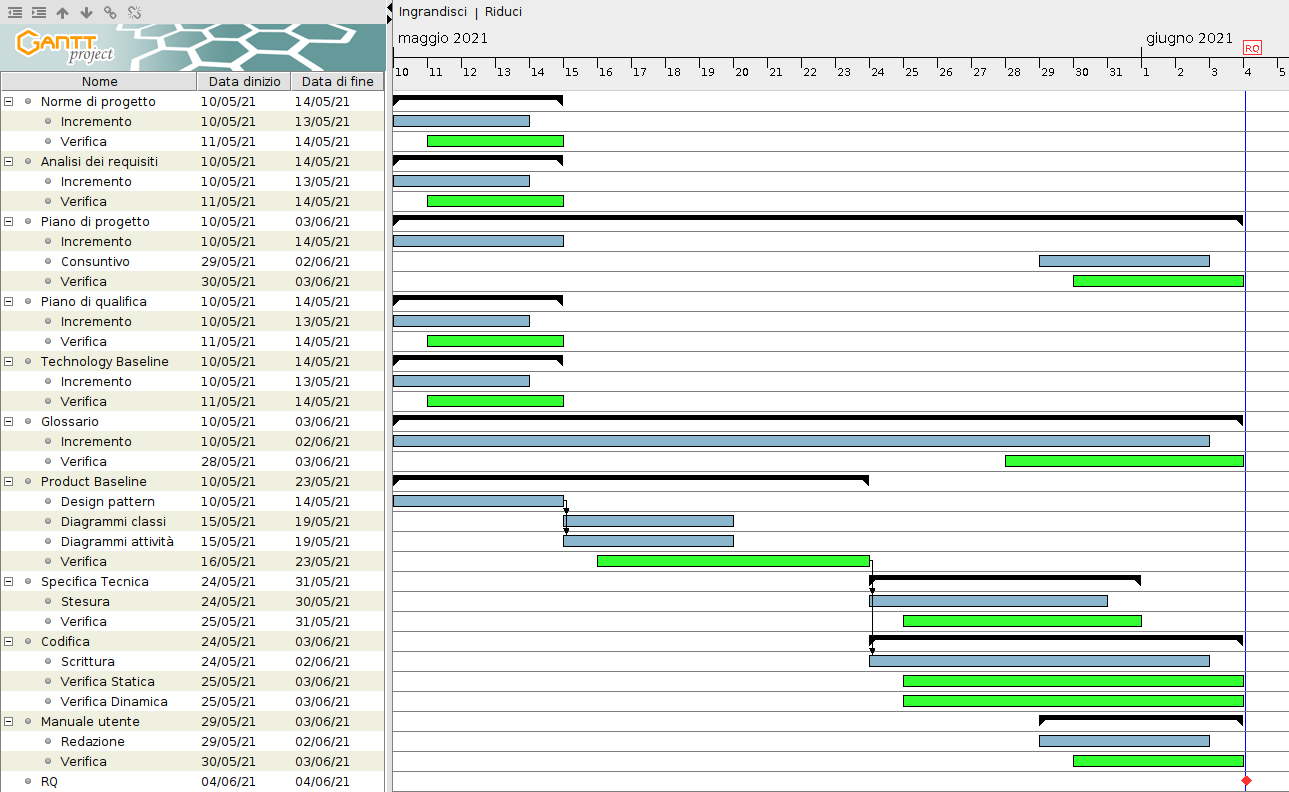
\includegraphics[scale=0.22]{../../../Images/Diagrammi/Gantt/progettazioneCodifica_v2.png}
    \centering
\end{figure}

\subsection{Validazione e collaudo}
\textit{Periodo: dal 2021-06-11 al 2021-07-02}\\
L'inizio di questa fase è il giorno della scadenza della \textit{Revisione di Qualifica} e la data di fine coincide con la data di consegna dei documenti in vista della \textit{Revisione di Accettazione}.\\
Le attività di questa fase sono:
\begin{itemize}
    \item \textbf{Incremento e verifica:} in cui i documenti precedentemente redatti vengono aggiornati e migliorati;
    \item \textbf{Validazione e collaudo:} per la parte di collaudo si eseguiranno ulteriori test sul prodotto, in modo da garantirne correttezza e stabilità. Per ciò che concerne la validazione, verrà valutata la coerenza del prodotto e dei requisiti specificati nel documento \textit{Analisi dei Requisiti} nella sua ultima versione;
\end{itemize}
\begin{figure}[!ht]
    \caption{Diagramma di Gantt dell'attività di Validazione e Collaudo}
    \vspace{5px}
    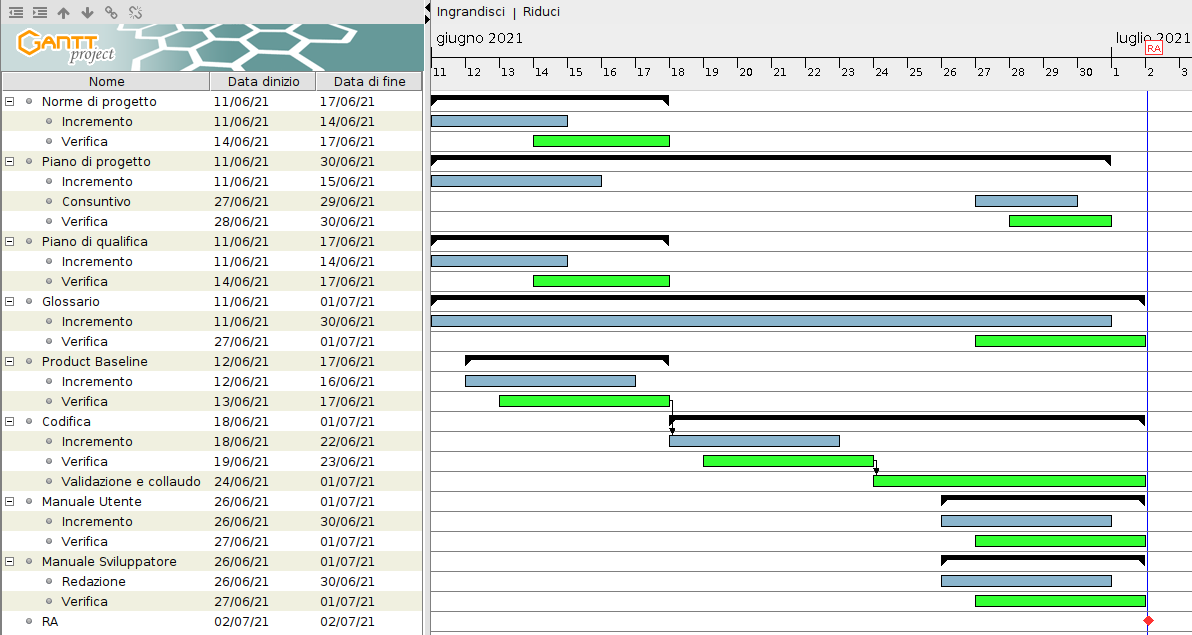
\includegraphics[scale=0.3]{../../../Images/Diagrammi/Gantt/validazione_v2.png}
    \centering
\end{figure}